% ==============================================================================
% EXPERIMENTOS
% ==============================================================================
% Instrucciones de la plantilla:
% - Detallar de manera clara y estructurada las pruebas realizadas.
% - Incluir tanto los resultados exitosos como los fallidos.
% - Detallar las variaciones exploradas en cada actividad.
% - Describir los experimentos base: objetivo, metodología empleada y resultados
%   obtenidos, respaldados con imágenes, gráficos o datos numéricos.
% ==============================================================================

\section{Experimentos}

En esta sección se describen las pruebas que hicimos con los dos objetos, en el orden en que las fuimos haciendo: los experimentos 1 a 6 corresponden a la casa y los 7 a 9, al planeta. Casi todas consisten en modificar el \textit{fragment shader} \texttt{11\_BasicPhongShader.fs} o los parámetros de las líneas 161 a 171 de \texttt{07\_IllumModels.cpp}, volver a compilar y observar el cambio. Los números de línea corresponden a la versión final de ambos archivos, que es la misma para los dos objetos.

% ------------------------------------------------------------------------------
\subsection{Experimento 1: componentes de Phong por separado}

\subsubsection{Objetivo del experimento}
Ver qué aporta cada componente del modelo de Phong agregándolas una por una al \textit{shader}, con la salida \texttt{FragColor = ex\_color}, es decir, sin la textura del modelo.

\subsubsection{Pruebas exitosas}
\textbf{Solo la componente ambiental.} Dejamos en \texttt{ex\_color} únicamente el término \texttt{K\_a * LightPower / (distance*distance)}. Con el valor por defecto de \texttt{material.ambient}, 0.2 en cada canal, el color es $0.2 \times 2.4 = 0.48$ en R, G y B, y la casa se dibuja como una silueta gris plana (Figura \ref{fig:exp_ambiental}). Como la componente ambiental no depende de la normal ni de la luz, todas las caras tienen exactamente el mismo color y no se distinguen las paredes, el techo ni el terreno: solo se reconoce el contorno.

\begin{figure}[H]
    \centering
    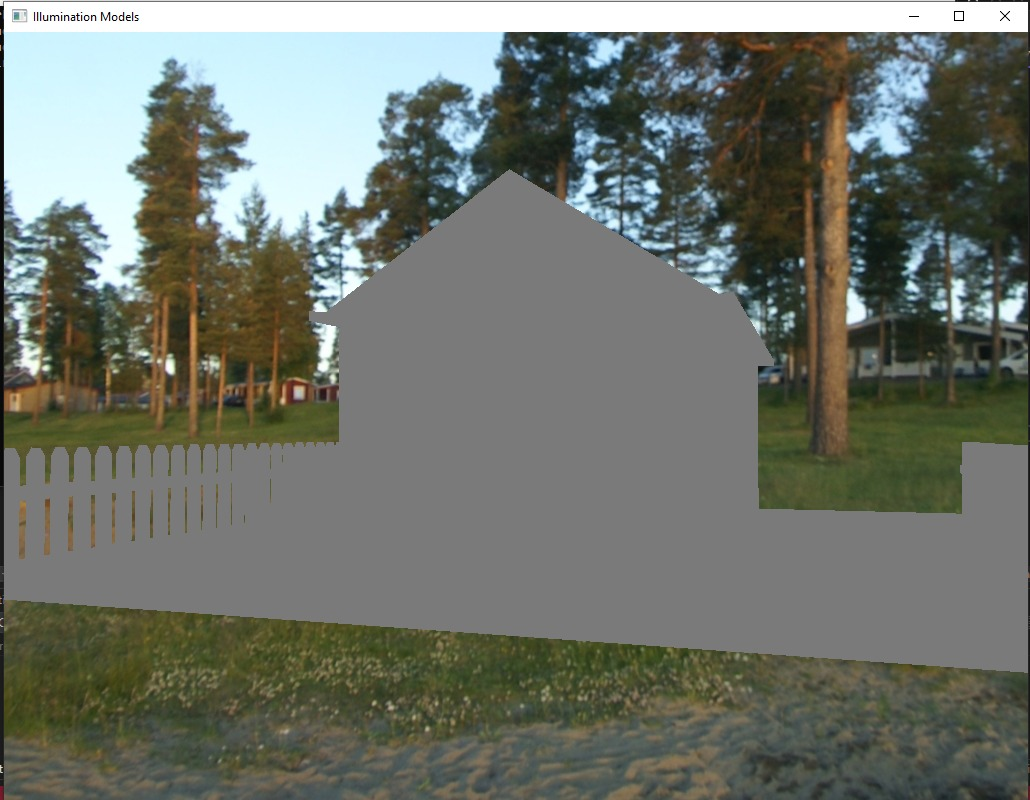
\includegraphics[width=0.65\textwidth]{Imagenes/Objeto1/objeto1e1.jpeg}
    \caption{Objeto 1 solo con la componente ambiental: todas las caras tienen el mismo gris y solo se distingue la silueta.}
    \label{fig:exp_ambiental}
\end{figure}

\textbf{Componente difusa.} En la línea 169 del \texttt{main} cambiamos el color difuso del material a un rojo oscuro, \texttt{glm::vec4(0.4f, 0.1f, 0.1f, 1.0f)}, y en el \textit{shader} descomentamos la línea 47, la del término \texttt{K\_d}. Para que compilara hubo que agregar el signo \texttt{+} al final de la línea 46 y mover el punto y coma al final de la 47. Con este cambio el terreno, cuya normal apunta hacia la luz, tomó un tono rosado, mientras que las caras que reciben la luz de lado o no la reciben conservaron el gris ambiental. Por primera vez se notó la diferencia de orientación entre las caras.

\textbf{Componente especular.} Repetimos el procedimiento con la línea 48, la del término \texttt{K\_s}, usando el color especular azul de la línea 170, \texttt{glm::vec4(0.1f, 0.1f, 0.8f, 1.0f)}. Apareció un brillo violeta sobre el terreno, en la zona donde el reflejo de la luz apunta hacia la cámara, y una línea del mismo color en la orilla del techo. Al mover la cámara el brillo cambia de lugar, cosa que no pasa con la componente difusa.

\textbf{Movimiento de la fuente.} Con las teclas Z, X, C y V movimos la luz alrededor de la casa. El brillo especular y las zonas rosadas de la componente difusa se desplazaron siguiendo al indicador de la luz, y al acercarla a una pared apareció sobre ella una mancha violeta. El brillo general de la escena no cambió con la distancia, porque el \textit{shader} atenúa con el \textit{uniform} \texttt{distance}, que es fijo, y no con la distancia real a la luz.

\subsubsection{Pruebas fallidas y análisis de errores}
\textbf{Componente ambiental saturada.} Al subir \texttt{material.ambient} a \texttt{glm::vec4(1.0f, 1.0f, 1.0f, 1.0f)} en la línea 168, la casa se volvió una silueta completamente blanca. El valor resultante es $1.0 \times 2.4 = 2.4$, y como el \textit{framebuffer} recorta cada canal a 1, todos los canales quedan en su máximo. Con la potencia de 60 y la distancia de 5, cualquier coeficiente ambiental mayor que $1/2.4 \approx 0.42$ satura el color, así que regresamos a valores pequeños.

% ------------------------------------------------------------------------------
\subsection{Experimento 2: textura del modelo}

\subsubsection{Objetivo del experimento}
Combinar la iluminación de Phong con las texturas que trae \texttt{House02.fbx}.

\subsubsection{Pruebas exitosas}
En la línea 54 del \textit{shader} cambiamos la salida de \texttt{FragColor = ex\_color} a \texttt{FragColor = texel * ex\_color}, donde \texttt{texel} es el color de la textura en las coordenadas del fragmento. La madera de las paredes, la teja del techo y el terreno aparecieron con su textura, teñidos por los colores del material: rojizos donde domina la componente difusa y violetas donde llega el brillo especular azul. La multiplicación escala el color de la textura canal por canal, de modo que un canal con poca luz oscurece esa parte del color del objeto.

% ------------------------------------------------------------------------------
\subsection{Experimento 3: potencia de la fuente}

\subsubsection{Objetivo del experimento}
Ver el efecto de la intensidad de la luz, \texttt{light.Power}, en la línea 164.

\subsubsection{Pruebas exitosas}
La potencia multiplica a las tres componentes, así que funciona como un control de brillo general. Con un valor bajo, la escena quedó casi a oscuras (Figura \ref{fig:exp_potencia}): las texturas apenas se distinguen y solo queda un reflejo tenue cerca del indicador de la luz, que en la captura está junto al techo. Al aumentar la potencia, la casa y el terreno recuperaron el color de sus texturas. Como el factor de atenuación es $L_i / r^2$, subir la potencia tiene el mismo efecto que acercar la luz, algo que en este programa no se puede hacer moviéndola porque la distancia del \textit{shader} es fija.

\begin{figure}[H]
    \centering
    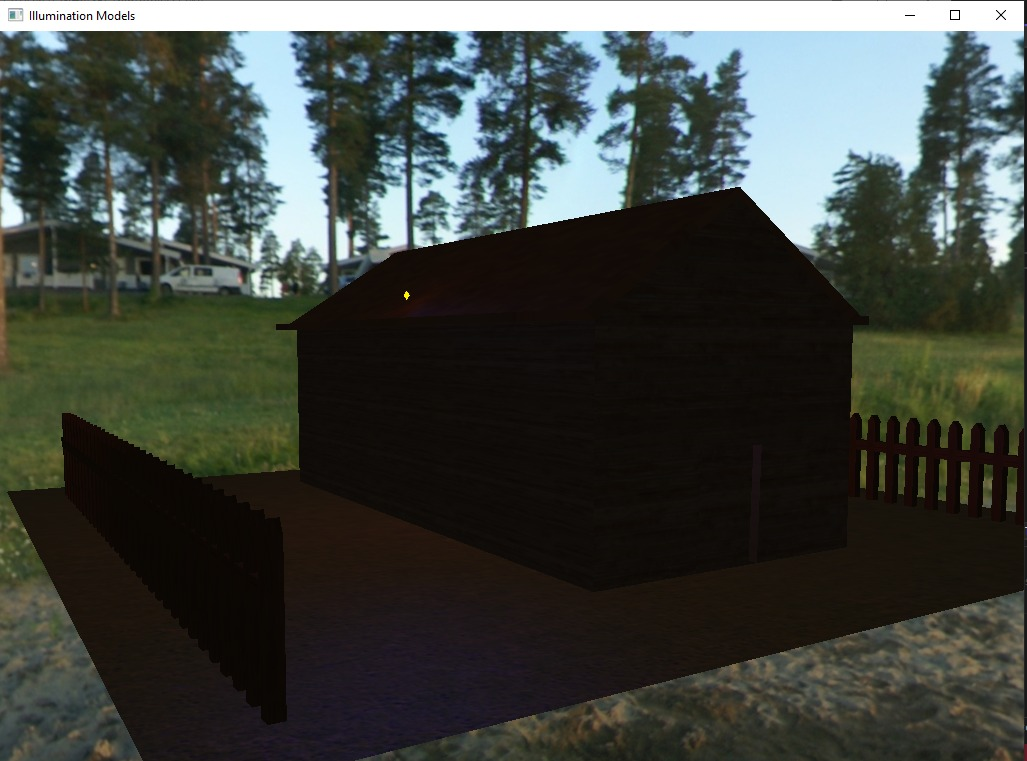
\includegraphics[width=0.65\textwidth]{Imagenes/Objeto1/objeto1e2.jpeg}
    \caption{Objeto 1 con poca potencia en la fuente de luz: la escena queda casi a oscuras.}
    \label{fig:exp_potencia}
\end{figure}

% ------------------------------------------------------------------------------
\subsection{Experimento 4: exponente especular}

\subsubsection{Objetivo del experimento}
Comprobar cómo cambia el brillo especular con el exponente $q$. En el programa, este exponente es \texttt{light.alphaIndex} (línea 165).

\subsubsection{Pruebas exitosas}
Al variar el exponente se confirmó lo que predice la Ecuación \ref{eq:phong}: mientras más alto es el valor, más pequeño y concentrado es el brillo especular, porque $(\cos\alpha)^q$ cae más rápido conforme el reflejo se aleja de la dirección del ojo. Con valores bajos el brillo se extiende sobre caras enteras.

\subsubsection{Pruebas fallidas y análisis de errores}
Para ver un brillo muy extendido escribimos \texttt{light.alphaIndex = 0.2;}. El resultado de la Figura \ref{fig:exp_alpha} no es el esperado: las caras que miran hacia el reflejo se tiñeron de un violeta uniforme y las demás quedaron completamente negras, separadas por una curva bien marcada sobre la pared de la casa.

\begin{figure}[H]
    \centering
    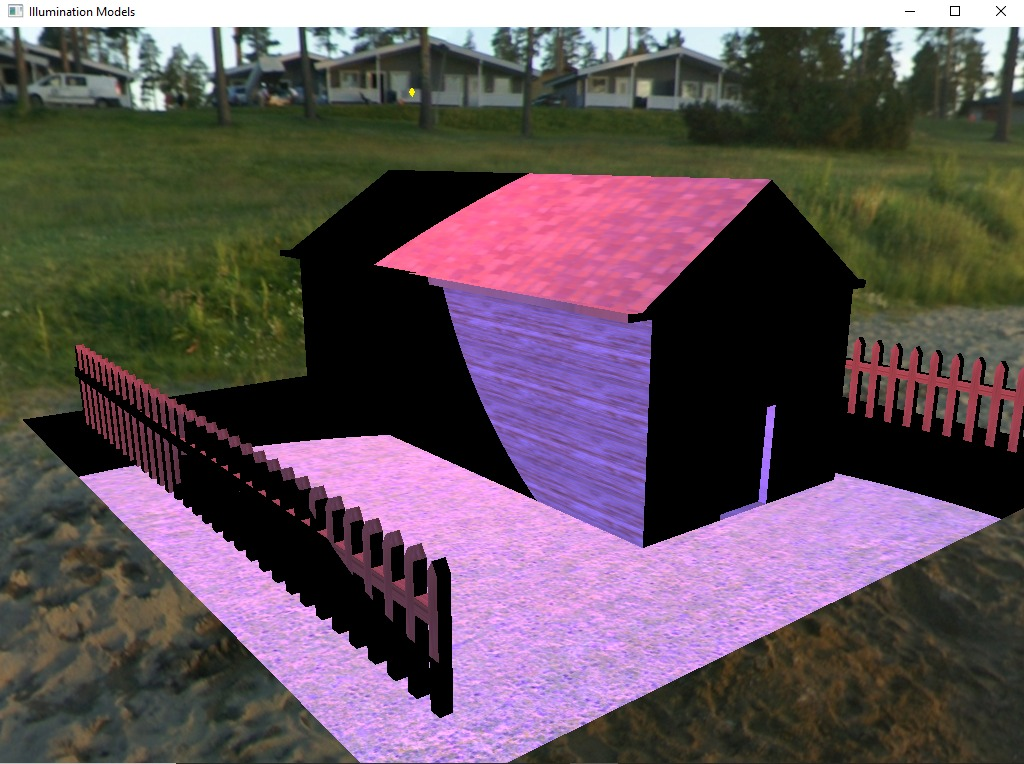
\includegraphics[width=0.65\textwidth]{Imagenes/Objeto1/objeto1e3.jpeg}
    \caption{Objeto 1 con \texttt{alphaIndex = 0.2}: caras violetas donde $\cos\alpha > 0$ y caras negras donde $\cos\alpha = 0$.}
    \label{fig:exp_alpha}
\end{figure}

La causa está en \texttt{light.h}, donde \texttt{alphaIndex} está declarado como \texttt{int}. El 0.2 se trunca a 0 al asignarlo, y en el \textit{shader} el término especular queda como \texttt{pow(cosAlpha, 0)}. Donde \texttt{cosAlpha} es positivo, la potencia vale 1 y se suma el color especular completo, $(0.1, 0.1, 0.8) \times 2.4$, que satura el azul y produce el violeta. Donde \texttt{cosAlpha} vale 0, porque el \texttt{clamp} recortó un coseno negativo, se calcula \texttt{pow(0, 0)}, que en GLSL no está definido. En nuestra tarjeta gráfica ese resultado invalidó la suma completa y los fragmentos salieron negros, aunque la componente ambiental y la difusa no fueran cero. La curva que separa las dos zonas es el lugar donde el reflejo de la luz es perpendicular a la dirección del ojo. Para usar valores de $q$ entre 0 y 1 habría que cambiar el tipo de \texttt{alphaIndex} a \texttt{float}, tanto en la clase como en el \textit{uniform}; en la versión final regresamos al valor de 10.

% ------------------------------------------------------------------------------
\subsection{Experimento 5: transparencia}

\subsubsection{Objetivo del experimento}
Hacer semitransparente la casa con el atributo \texttt{material.transparency}.

\subsubsection{Pruebas exitosas}
Agregamos en la línea 171 \texttt{material.transparency = 0.5;}, que el \textit{shader} copia en el canal alfa de \texttt{ex\_color}. Como la mezcla con \texttt{GL\_SRC\_ALPHA} y \texttt{GL\_ONE\_MINUS\_SRC\_ALPHA} ya estaba activada en \texttt{Update()}, cada fragmento de la casa se combinó a partes iguales con lo que había detrás. En la Figura \ref{fig:exp_transparencia}, tomada todavía con \texttt{alphaIndex = 0.2}, a través de las paredes se ven la cerca del fondo, el interior del techo y el cubemap, y las caras que antes eran negras ahora son grises oscuras y translúcidas.

\begin{figure}[H]
    \centering
    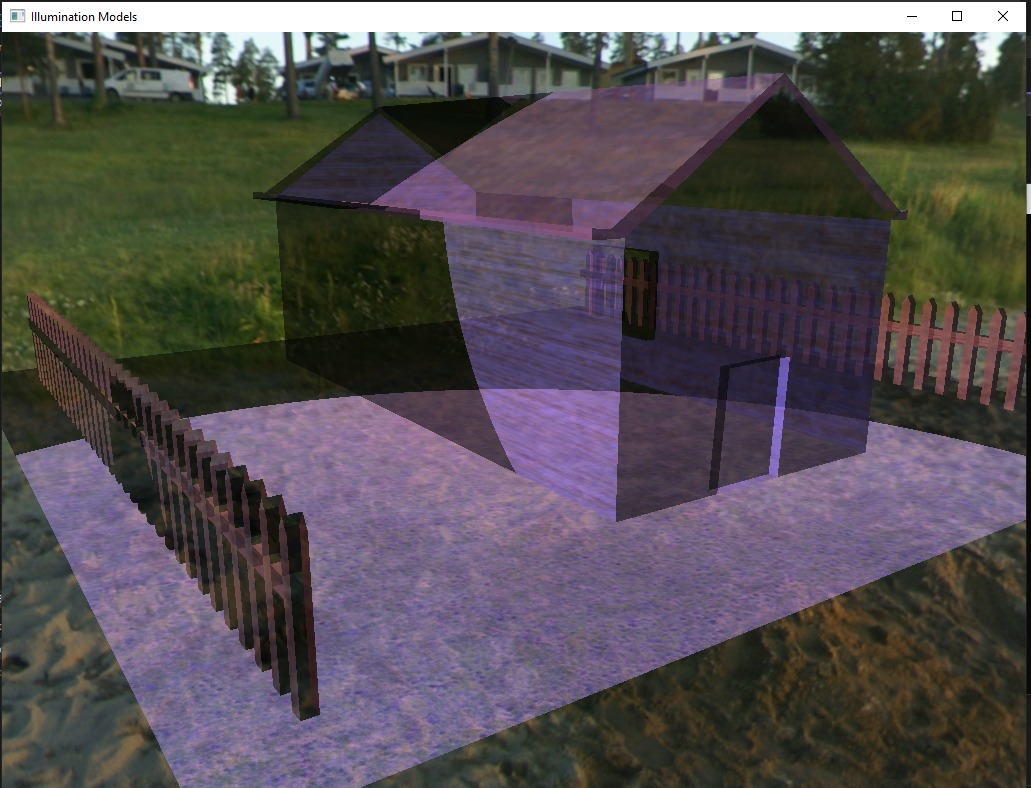
\includegraphics[width=0.65\textwidth]{Imagenes/Objeto1/objeto1e4.jpeg}
    \caption{Objeto 1 con \texttt{transparency = 0.5}: a través de las paredes se ven la cerca y el fondo.}
    \label{fig:exp_transparencia}
\end{figure}

% ------------------------------------------------------------------------------
\subsection{Experimento 6: música de fondo}

\subsubsection{Objetivo del experimento}
Reproducir una pista de audio mientras se ejecuta la escena.

\subsubsection{Pruebas fallidas y análisis de errores}
En el código del laboratorio, la línea 176 llamaba a \texttt{play2D} con la ruta \texttt{sound/EternalGarden.mp3}, pero en \texttt{bin} no existían la carpeta \texttt{sound} ni ese archivo, así que al ejecutar no había nada que reproducir. El código compila igual, porque la ruta solo se usa en tiempo de ejecución; la falta del archivo no se nota hasta abrir el programa.

\subsubsection{Pruebas exitosas}
Creamos la carpeta \texttt{sound} dentro de \texttt{bin} y descargamos ahí la pista \textit{Carefree} de Kevin MacLeod \cite{macleod_carefree}, un MP3 estéreo de 256 kbps a 44.1 kHz. La elegimos porque se distribuye con licencia Creative Commons Atribución 4.0, que permite usarla dando crédito al autor; por eso el crédito aparece en un comentario de la misma línea y en las referencias. Después cambiamos la ruta de la línea 176 a \texttt{sound/Carefree.mp3}. La ruta es relativa al directorio de trabajo, que es \texttt{bin}, y el segundo argumento, \texttt{true}, hace que la pista se repita en bucle. Al compilar y ejecutar, el programa abrió sin errores y la música empezó a sonar con la ventana. irrKlang lee el MP3 con el complemento \texttt{ikpMP3.dll}, que ya estaba en \texttt{bin}.

% ------------------------------------------------------------------------------
\subsection{Experimento 7 (Objeto 2): el planeta con los parámetros del Objeto 1}

\subsubsection{Objetivo del experimento}
Comprobar que el planeta exportado se carga con el \texttt{model.h} de esta práctica y ver cómo se ve con los parámetros que dejamos para la casa.

\subsubsection{Pruebas exitosas}
En la práctica 6, la esfera cerraba el programa porque Assimp la entregaba sin normales, y lo resolvimos agregando \texttt{aiProcess\_GenSmoothNormals} al cargador. El \texttt{model.h} de esta práctica no tiene esa bandera, así que la primera prueba fue cambiar solo la ruta del modelo (línea 146) y la cámara (línea 50). El programa abrió sin errores y el planeta mostró un degradado de iluminación, lo que confirma que el FBX que exportamos de nuevo con Blender 5.2 sí trae las normales.

\subsubsection{Pruebas fallidas y análisis de errores}
Con la luz en $(0, 5, 0)$, el material rojizo y azul y la transparencia de 0.5, el resultado de la Figura \ref{fig:o2_params_obj1} no sirve para un planeta. La luz está justo arriba, así que solo el hemisferio norte recibe componente difusa y el brillo violeta queda en el borde superior, sobre Norteamérica. Además, la mitad izquierda del planeta es mucho más transparente que la derecha. Es el mismo problema de orden de dibujo que vimos en el techo de la casa: los triángulos de la esfera se dibujan en el orden en que están en la malla. Donde un triángulo del hemisferio trasero se dibuja antes que el delantero, los dos se mezclan con el fondo y el resultado es más opaco. Donde el delantero va primero, escribe su profundidad, el trasero se descarta y solo queda una capa.

\begin{figure}[H]
    \centering
    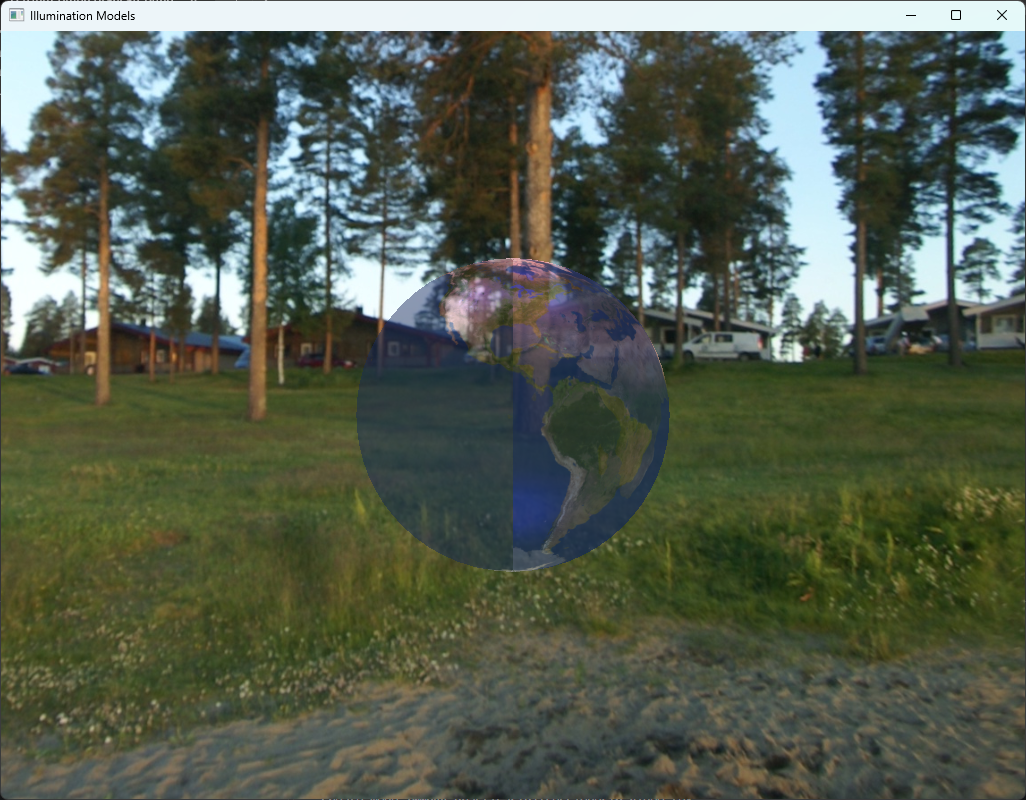
\includegraphics[width=0.65\textwidth]{Imagenes/Objeto2/objeto2e1.png}
    \caption{El planeta con los parámetros del Objeto 1: luz desde arriba, brillo violeta en el borde y la mitad izquierda más transparente que la derecha.}
    \label{fig:o2_params_obj1}
\end{figure}

Por eso cambiamos la luz, el material y la transparencia a los valores del Listado \ref{lst:parametros_objeto2}, con los que se obtuvo la Figura \ref{fig:objeto2}.

% ------------------------------------------------------------------------------
\subsection{Experimento 8 (Objeto 2): exponente especular con valores enteros}

\subsubsection{Objetivo del experimento}
Repetir la prueba del exponente especular que falló con el Objeto 1, ahora con valores enteros que \texttt{alphaIndex} sí puede guardar.

\subsubsection{Pruebas exitosas}
Compilamos el programa con \texttt{light.alphaIndex} igual a 1, 10 y 100, sin cambiar nada más. La Figura \ref{fig:o2_alpha} compara los tres resultados. Con 1, el término $(\cos\alpha)^1$ decae despacio y el brillo se reparte sobre casi todo el lado de día, que se ve más claro que con los otros valores. Con 10 el brillo es una mancha sobre el Caribe, y con 100 se reduce a un punto pequeño en el mismo lugar. El centro del brillo queda en el mismo lugar en las tres imágenes, porque depende solo de dónde el reflejo de la luz apunta al ojo; el exponente cambia únicamente su tamaño. En la casa, la prueba con 0.2 falló y las caras planas no dejaban ver bien el brillo; en la esfera se aprecia con claridad que, mientras más alto el exponente, más pequeño y concentrado es el brillo.

\begin{figure}[H]
    \centering
    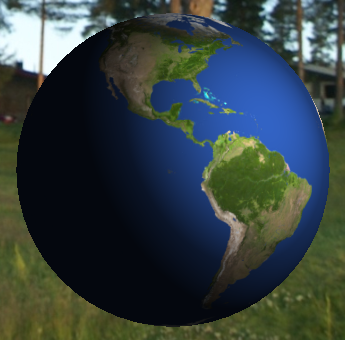
\includegraphics[width=0.32\textwidth]{Imagenes/Objeto2/objeto2e2a.png}
    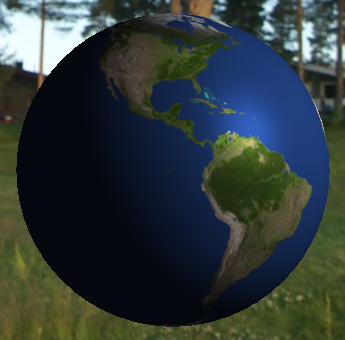
\includegraphics[width=0.32\textwidth]{Imagenes/Objeto2/objeto2e2b.png}
    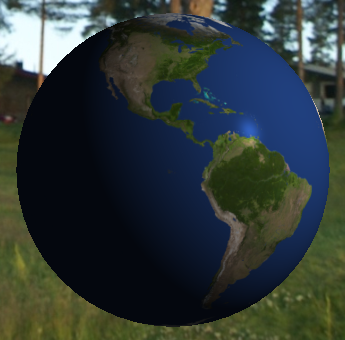
\includegraphics[width=0.32\textwidth]{Imagenes/Objeto2/objeto2e2c.png}
    \caption{El planeta con \texttt{alphaIndex} igual a 1 (izquierda), 10 (centro) y 100 (derecha).}
    \label{fig:o2_alpha}
\end{figure}

En las tres imágenes el brillo sobre el mar es azul claro y no blanco. El \textit{shader} multiplica toda la iluminación por la textura (\texttt{FragColor = texel * ex\_color}), incluida la componente especular, así que el reflejo toma el color de la superficie. Para un océano esto no es realista, porque el reflejo del Sol sobre el agua se ve blanco.

% ------------------------------------------------------------------------------
\subsection{Experimento 9 (Objeto 2): color de la luz}

\subsubsection{Objetivo del experimento}
Ver el efecto de \texttt{light.Color} (línea 163), que multiplica a las tres componentes.

\subsubsection{Pruebas exitosas}
Cambiamos la luz blanca por una anaranjada, \texttt{glm::vec4(1.0f, 0.6f, 0.3f, 1.0f)}, parecida a la de un atardecer. Los continentes se tiñeron de naranja y café, pero los océanos quedaron casi negros (Figura \ref{fig:o2_luz}). El mar de la textura es azul, con poco rojo y verde, y la luz tiene solo 0.3 de azul, así que el producto canal por canal es pequeño en los tres canales. En el modelo de Phong, una superficie solo puede reflejar los colores que tiene la luz que le llega. El brillo especular también se volvió anaranjado y casi desapareció sobre el mar.

\begin{figure}[H]
    \centering
    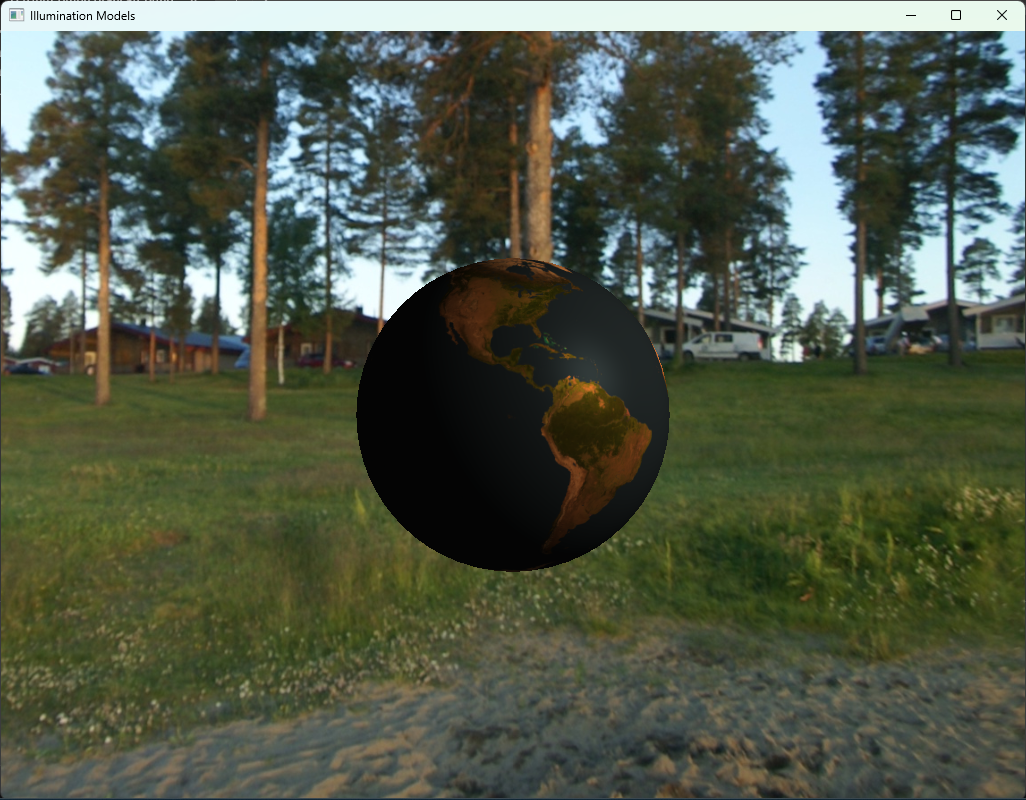
\includegraphics[width=0.65\textwidth]{Imagenes/Objeto2/objeto2e3.png}
    \caption{El planeta con luz anaranjada $(1, 0.6, 0.3)$: los continentes se ven naranjas y los océanos casi negros.}
    \label{fig:o2_luz}
\end{figure}

Después de esta prueba regresamos a la luz blanca y dejamos el exponente en 30, un punto intermedio entre la mancha de 10 y el punto de 100.
